\documentclass{beamer}

\usetheme{LANL}
\usepackage{graphicx}
\graphicspath{{./figs/}}

\definecolor{myLightGray}{RGB}{192,192,192}
\setbeamercolor{fakegraphic}{bg=myLightGray,fg=black}

\title{OpenMPIR}
\subtitle{Implementing OpenMP tasks with Tapir}

\author[shortname]{\underline{George Stelle} \inst{1} \and William S. Moses \inst{2} \\ Stephen L. Olivier \inst{3} \and Patrick M\raise .40ex\hbox{c}Cormick \inst{1}}
\institute[shortinst]{\inst{1} Los Alamos National Laboratory \and %
                      \inst{2} MIT CSAIL \and
                      \inst{3} Sandia National Laboratories}
          
\date{November 13, 2017}

\begin{document}

\begin{frame}
\maketitle
\end{frame}

\begin{frame}
\frametitle{Outline}
\begin{itemize}
\item OpenMP
\item Motivation
\item Tapir
\item Implementation
\item Results
\item Discussion
\item Questions
\end{itemize}
\end{frame}

\begin{frame}[fragile]
\frametitle{OpenMP}
\begin{verbatim}
int fib(int n){                   
  if (n < 2)
    return n;
  else {
    int x, y;
    #pragma omp task
      x = fib(n-1);  
    #pragma omp task
      y = fib(n-2);  
    #pragma omp taskwait
    return x+y;   
  }
}
\end{verbatim}
\end{frame}

\begin{frame}[fragile]
\frametitle{OpenMP LLVM IR}
\begin{verbatim}
...
  %19 = call i32 @__kmpc_omp_task(%ident_t* nonnull @0, i32 %5, i8* %10) #2
  %20 = call i8* @__kmpc_omp_task_alloc(%ident_t* nonnull @0, i32 %5, i32 1, i64 48, i64 16, i32 (i32, i8*)* bitcast (i32 (i32, %struct.kmp_task_t_with_privates.1*)* @.omp_task_entry..3 to i32 (i32, i8*)*)) #2
  %21 = bitcast i8* %20 to i8**
  %22 = load i8*, i8** %21, align 8, !tbaa !8
...
  %28 = load i32, i32* %2, align 4, !tbaa !4
  store i32 %28, i32* %27, align 4, !tbaa !13
  %29 = call i32 @__kmpc_omp_task(%ident_t* nonnull @0, i32 %5, i8* %20) #2
  %30 = call i32 @__kmpc_omp_taskwait(%ident_t* nonnull @0, i32 %5) #2
...
\end{verbatim}
\end{frame}

\begin{frame}[fragile]
\begin{figure}
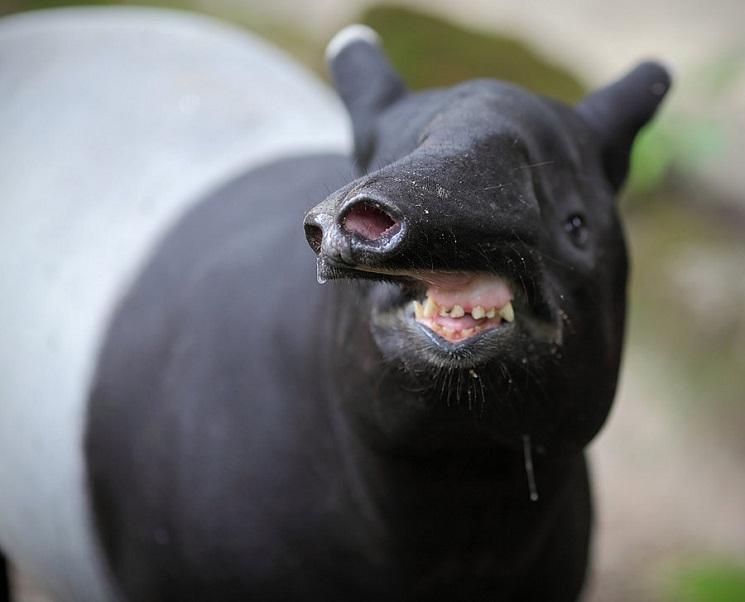
\includegraphics[width=0.8\linewidth]{tapir.jpg}
\end{figure}
\end{frame}

\begin{frame}[fragile]
\frametitle{Tapir}
\begin{center}
\huge{\texttt{detach \\ reattach \\ sync}}
\end{center}
\end{frame}

\begin{frame}[fragile]
\begin{tabular*}{\linewidth}{ll}
\begin{minipage}[T]{0.4\linewidth}
\begin{verbatim}
int fib(int n){                   
...
    #pragma omp task
      x = fib(n-1);  
    #pragma omp task
      y = fib(n-2); 
    #pragma omp taskwait
...
}
\end{verbatim}
\end{minipage}
  &
\begin{minipage}[T]{0.6\linewidth}
{\scriptsize
\begin{verbatim}
...
if.end:
  detach label %det.achd, label %det.cont

det.achd:
  %2 = load i32, i32* %n.addr, align 4
  %sub = sub nsw i32 %2, 1
  %call = call i32 @fib(i32 %sub)
  store i32 %call, i32* %x, align 4
  reattach label %det.cont

det.cont:
  detach label %det.achd1, label %det.cont4

det.achd1:
  %3 = load i32, i32* %n.addr, align 4
  %sub2 = sub nsw i32 %3, 2
  %call3 = call i32 @fib(i32 %sub2)
  store i32 %call3, i32* %y, align 4
  reattach label %det.cont4

det.cont4:
  sync label %sync.continue
...
\end{verbatim}
}
\end{minipage}
\end{tabular*}
\end{frame}

\begin{frame}[fragile]
\frametitle{Overview}
\begin{figure}
\vspace{-1cm}
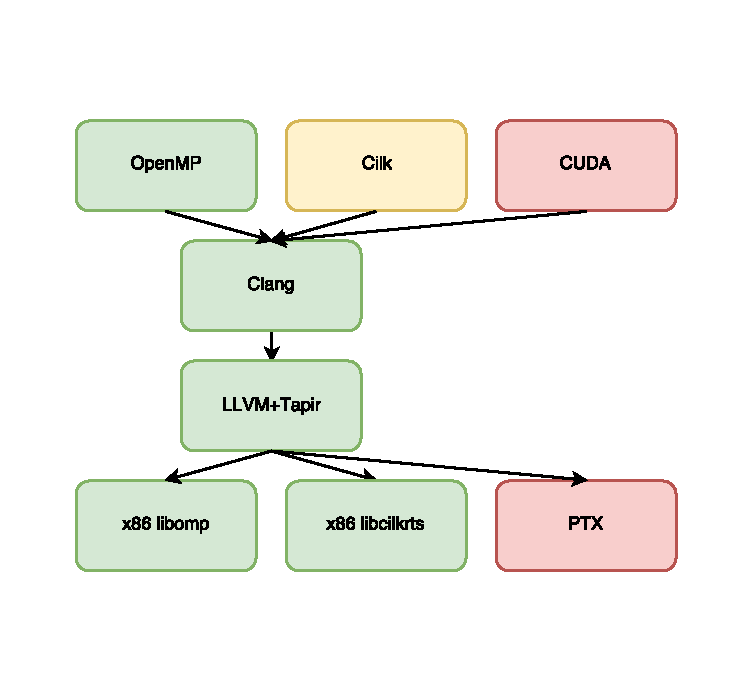
\includegraphics[width=0.6\linewidth]{tapir-io}
\end{figure}
\end{frame}

\begin{frame}[fragile]
\frametitle{Results}
\begin{figure}
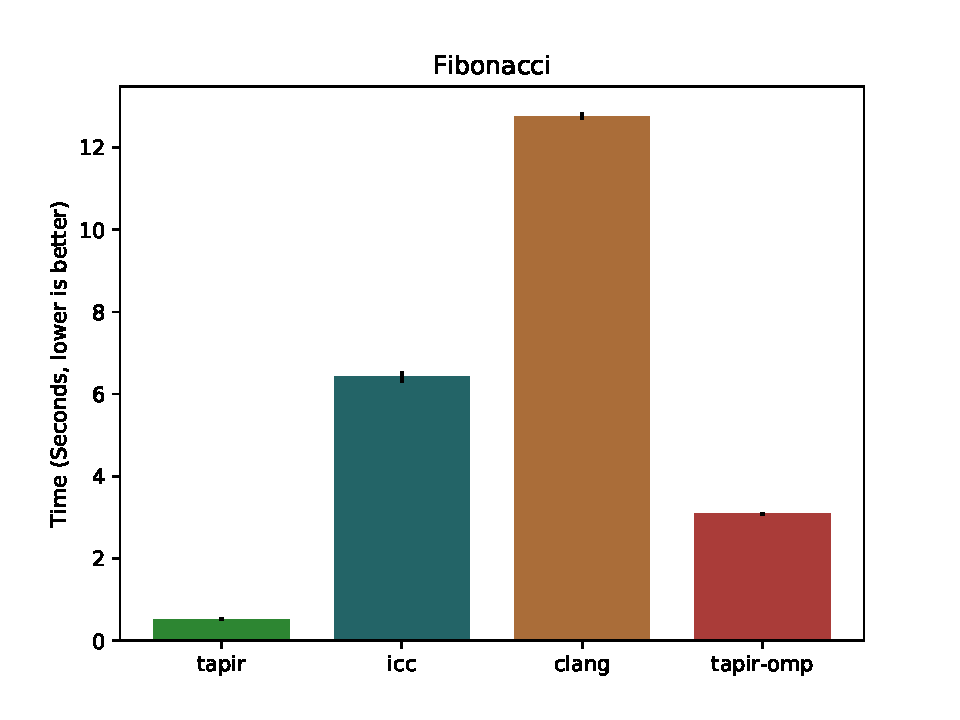
\includegraphics[width=0.7\linewidth]{fib}
\end{figure}
\end{frame}

\begin{frame}[fragile]
\frametitle{Results}
\begin{figure}
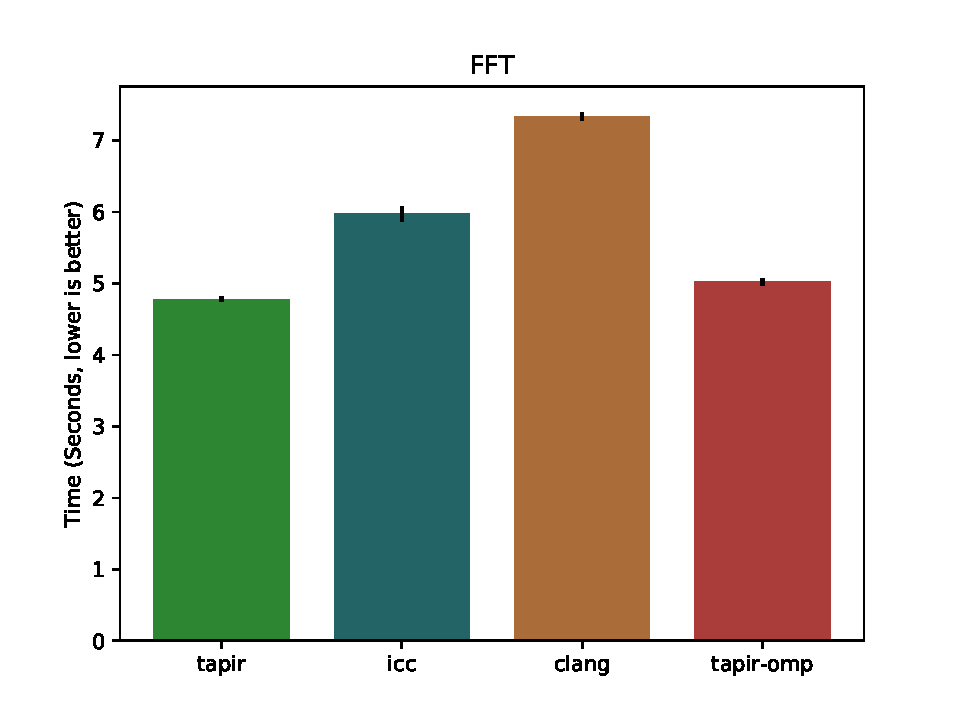
\includegraphics[width=0.7\linewidth]{fft}
\end{figure}
\end{frame}

\begin{frame}[fragile]
\frametitle{Results}
\begin{figure}
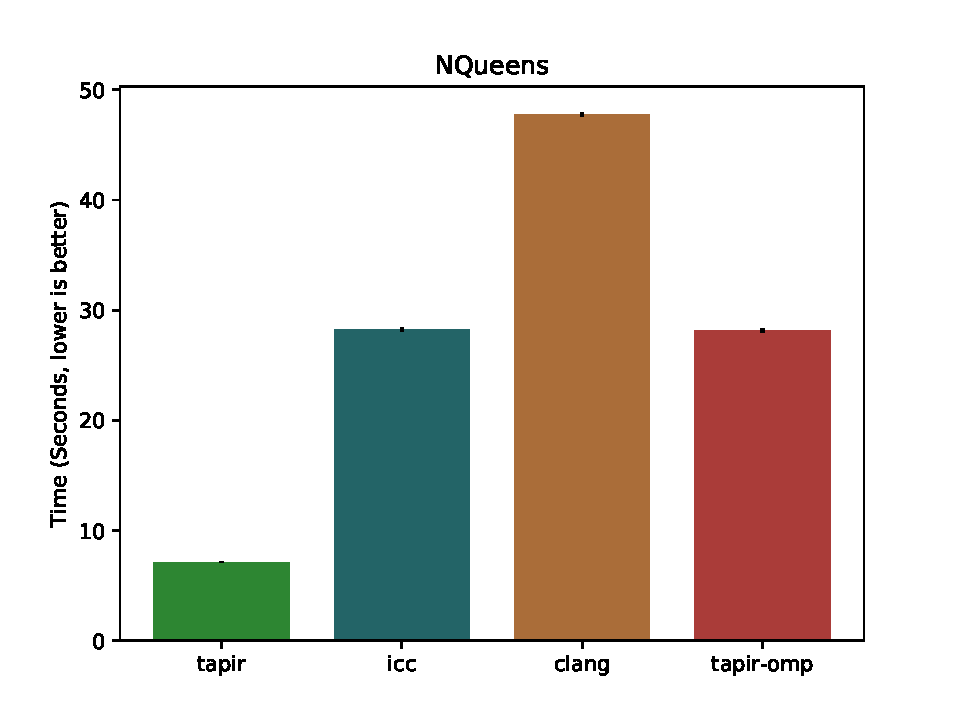
\includegraphics[width=0.7\linewidth]{nqueens}
\end{figure}
\end{frame}

\begin{frame}
\begin{center}
\huge{The other 355 pages?}
\end{center}
\end{frame}

\begin{frame}[fragile]
\frametitle{Questions?}
\begin{figure}
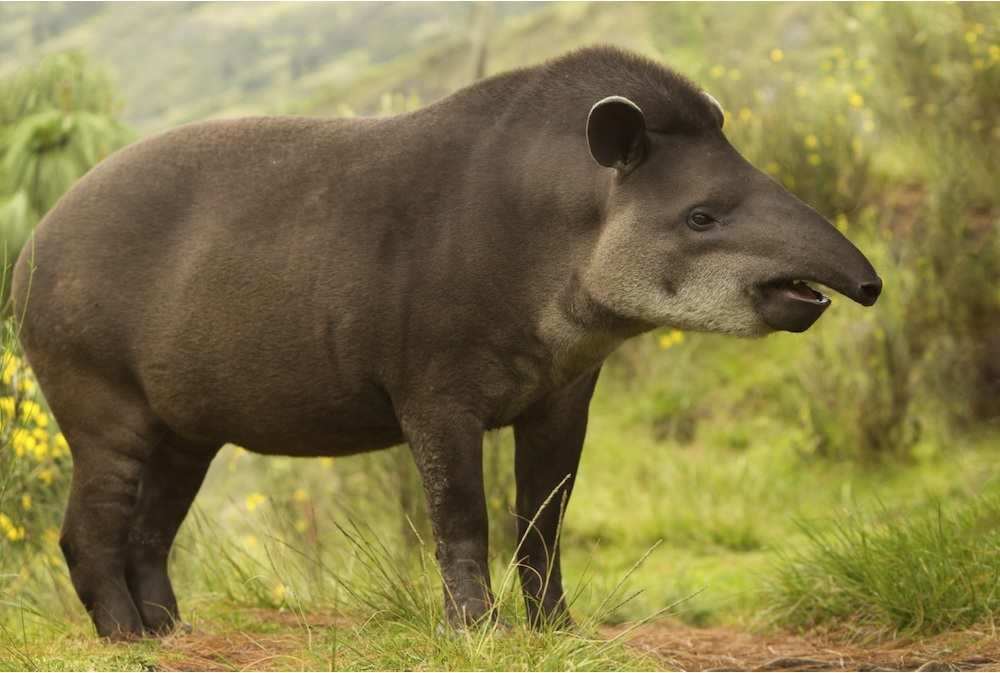
\includegraphics[width=0.8\linewidth]{tapir-side.jpg}
\end{figure}
\end{frame}

\begin{frame}[fragile]
\frametitle{Acknowledgements}
This research was supported by the Exascale Computing Project (17-SC-20-SC), a joint project of the U.S. Department of Energy’s Office of Science and National Nuclear Security Administration, responsible for delivering a capable exascale ecosystem, including software, applications, and hardware technology, to support the nation’s exascale computing imperative.
\end{frame}
\end{document}

